\documentclass[a4paper]{report}
\author{Jure Kos}
\title{Vaja 13, Bernoullijeva enačba}
\date{20.12.2021}
\usepackage{graphicx}
\graphicspath{ {./images/} }

\begin{document}

\maketitle

\chapter*{Uvod}
Pri stacionarnem gibanju nestisljive tekočine v cevi pojema zaradi viskoznosti in upora vsota tlaka ter povprečne gostote potencialne in kinetične energije v smeri toka. Za približen izračun si predstavljamo, da je hitrost po vsem preseku enaka in zapišemo:

\[p_1+\rho gz_1+\frac{1}{2}\rho v_{s1}^2 > p_2+\rho gz_2+\frac{1}{2}\rho v_{s2}^2\]

Povprečna hitrost $v_s$ je enaka $\Phi/S$, kjer je prostorninski tok, ki se vzdolž cevi ne spreminja, S pa je presek cevi na določenem mestu. Če mesti 1 in 2 med seboj nista preveč oddaljeni, smemo za približne račune neenačbo nadomestiti z Bernoullijevo enačbo:

\[p_1+\rho gz_1+\frac{1}{2}\rho v_{s1}^2 = p_2+\rho gz_2+\frac{1}{2}\rho v_{s2}^2\]

ki je posebna oblika izreka o kinetični energiji. Za vodoravno cev $(z1 = z2)$ velja v takem primeru:

\[p_1-p_2=\frac{1}{2}(\rho v_{s2}^2-\rho v_{s1}^2)=\frac{1}{2}\rho\left(\frac{1}{S_2^2}-\frac{1}{S_1^2}\right)\Phi^2=k\Phi^2\]

Razlika tlakov je torej sorazmerna s kvadratom prostorninskega toka. Cev s spre-
menljivim presekom (Venturijeva cev) zato s pridom rabimo za merjenje prostorninskega toka. Pri tem merimo tlačno razliko, medtem ko konstanto k za dano Venturijevo cev enkrat za vselej izračunamo ali izmerimo. Pri naši vaji merimo tlačno razliko z živosrebrnim manometrom: 

\[\Delta p=(\rho'-\rho_v g \Delta h\]

kjer je $\delta h$ razlika gladin živega srebra v krakih manometra, $\rho'$ gostota živega srebra in $\rho_v$ gostota vode. Zato zapišemo:

\[\Phi=K\sqrt{\Delta h}\]

kjer je $K^2=(\rho'-\rho_v)g/k$


\section{Naloga}
Določiti prostorninski tok vode z Venturijevo cevjo in ga primerjati z direktno izmerjenim.

\section{Potrebščine}
1. Premična posoda (rezervoar) z dovodno in dvema odvodnima cevema,\\
2. Venturijeva cev ($d_2=6,0mm$, $d_1=12,8mm$) z dvema manometroma,\\
3. menzura,\\
4. štoparica (na telefonu).

\chapter*{Potek}
Naprava za preizkus Bernoullijeve enačbe je sestavljena iz rezervoarja, pritrjenega
na vodilu ob steni, iz Venturijeve cevi in treh gumijevih cevi, s katerimi dovajamo in
odvajamo vodo iz rezervoarja.\\

\begin{figure}[h]
\centering
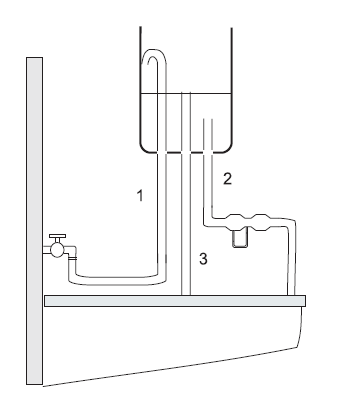
\includegraphics[width=8cm]{Skica}
\end{figure}

Cev 1 je dovodna cev in je priključena na vodovodno pipo, cevi 2 in 3 pa sta odvodni cevi. Cev 2 je priključena na Venturijevo cev, cev 3 pa vodi direktno v odtočni lijak. Dotok vode naravnamo pri vseh meritvah tako, da sega gladina vode v rezervoarju do ustja cevi 3 in voda tako ves čas odteka tudi direktno v lijak. S tem zmanjšamo nihanje vodne gladine, ki bi lahko nastopilo zaradi sprememb tlaka v vodovodnem omrežju. Pritrdimo rezervoar v najnižjo lego in počasi odpiramo vodovodno pipo, dokler ne začne teči voda iz rezervoarja tudi skozi cev 3. Počakamo nekaj časa, da voda, ki teče skozi Venturijevo cev, izpodrine ves zrak. Še enkrat kontroliramo, če je vodni tok dovolj močan tako, da voda odteka tudi po cevi 3 in začnemo z meritvijo. Na manometru Venturijeve cevi odčitamo tlačno razliko $\Delta h$ in nato še direktno izmerimo prostorninski tok! Pod iztočno cev podstavimo steklenico in natočimo vodo do značke (prostornina je podana). Izmerimo čas natakanja vsaj trikrat. Vse meritve ponovimo še pri srednji in najvišji legi rezervoarja. Za vsako lego rezervoarja izračunamo povprečni tok $\Phi = V\overline{t}$, kjer je V prostornina natočene vode in $\overline{t}$ povprečni čas natakanja, in povprečno tlačno razliko $\overline{\Delta h}$. S podatki za Venturijevo cev izračunamo konstanto K, potem pa iz povprečne tlačne razlike $\Delta h$ po enačbi izračunamo vodni tok v vseh treh primerih. Primerjamo ga z direktno izmerjenim.

\chapter*{Računi}
Z enačbo za volumski pretok izračunamo volumske pretoke za vseh 6 meritev.

\[\Phi=\frac{V}{\overline{t}}\]

Dobimo naslednje pretoke:
\begin{center}
\begin{tabular}{ |c|c| } 
 \hline
 1&0,0651$m^3/s\pm0,00181m^3/s$\\
 2&0,0596$m^3/s\pm0,00068m^3/s$\\
 3&0,0542$m^3/s\pm0,00100m^3/s$\\
 4&0,0469$m^3/s\pm0,00075m^3/s$\\
 5&0,0403$m^3/s\pm0,00099m^3/s$\\
 6&0,0321$m^3/s\pm0,00055m^3/s$\\
 \hline
\end{tabular}
\end{center}

Konstanto k izračunamo po enačbi

\[k=\frac{1}{2}\rho\left(\frac{1}{S_2^2}-\frac{1}{S_1^2}\right)=5,95\cdot 10^{11}kg/m^7\]

Vstavimo jo v enačbo in izračunamo K

\[K=\sqrt{(\rho'-\rho_v)g/k}=4,55 \cdot 10^{-4}\frac{m^{\frac{5}{2}}}{s}\]

Nato pretoke izračunamo še preko razlike tlakov po enačbi

\[\Phi=K\sqrt{\Delta h}\]

Dobimo naslednje pretoke:
\begin{center}
\begin{tabular}{ |c|c| } 
 \hline
 1&0,0875$m^3/s\cdot(1\pm 0,0135)m^3/s$\\
 2&0,0801$m^3/s\cdot(1\pm 0,0161)m^3/s$\\
 3&0,0734$m^3/s\cdot(1\pm 0,0192)m^3/s$\\
 4&0,0643$m^3/s\cdot(1\pm 0,0250)m^3/s$\\
 5&0,0576$m^3/s\cdot(1\pm 0,0313)m^3/s$\\
 6&0,0477$m^3/s\cdot(1\pm 0,0455)m^3/s$\\
 \hline
\end{tabular}
\end{center}


Skupna tabela razultatov je
\begin{center}
\begin{tabular}{ |c|c|c| } 
 \hline
 $\Delta h$ & Izmerjeni pretoki & Izračunani pretoki\\
 \hline
 0,037m & 0,0651$m^3/s\cdot(1\pm 0,0278)m^3/s$ & 0,0875$m^3/s\cdot(1\pm 0,0135)m^3/s$\\
 0,031m & 0,0596$m^3/s\cdot(1\pm 0,0114)m^3/s$ & 0,0801$m^3/s\cdot(1\pm 0,0161)m^3/s$\\
 0,026m & 0,0542$m^3/s\cdot(1\pm 0,0185)m^3/s$ & 0,0734$m^3/s\cdot(1\pm 0,0192)m^3/s$\\
 0,02m & 0,0469$m^3/s\cdot(1\pm 0,0159)m^3/s$ & 0,0643$m^3/s\cdot(1\pm 0,0250)m^3/s$\\
 0,016m & 0,0403$m^3/s\cdot(1\pm 0,0246)m^3/s$ & 0,0576$m^3/s\cdot(1\pm 0,0313)m^3/s$\\
 0,011m & 0,0321$m^3/s\cdot(1\pm 0,0172)m^3/s$ & 0,0477$m^3/s\cdot(1\pm 0,0455)m^3/s$\\
 \hline
\end{tabular}
\end{center}

\chapter*{Grafi}
Graf ki ga narišemo za izračun izmerjenega K.\\

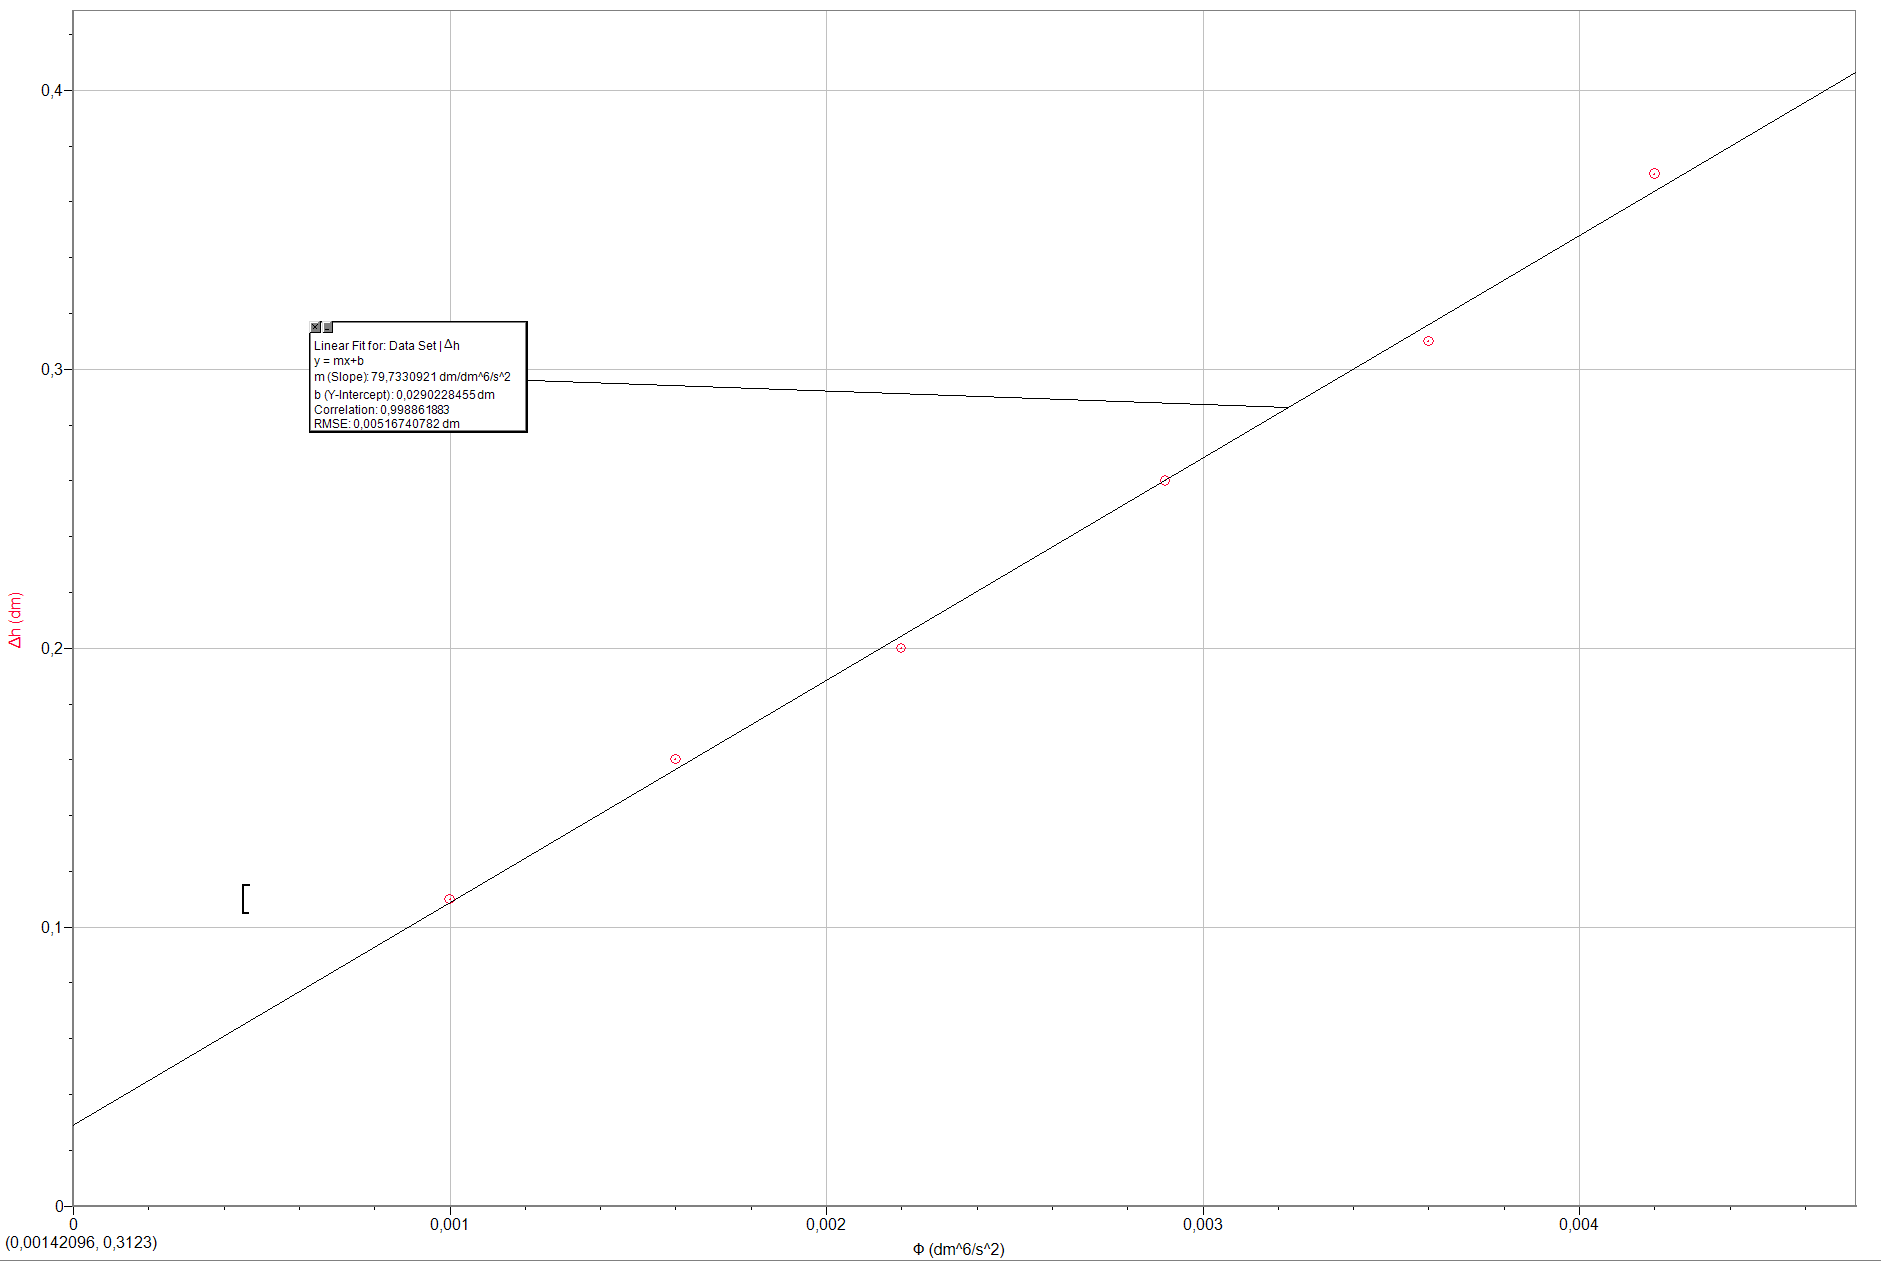
\includegraphics[width=\textwidth]{Graf}

Če iz naklona grafa izračunamo K po formuli

\[K=\frac{1}{\sqrt{k}}\]

dobimo \[k_{izmerjeni}=4,4\cdot 10^{-4} \cdot 10^{-4}\frac{m^{\frac{5}{2}}}{s}\pm 0,2\cdot 10^{-4}\cdot 10^{-4}\frac{m^{\frac{5}{2}}}{s}\]


\end{document}